\documentclass[12pt]{report}
\usepackage[francais]{babel}
\usepackage{ucs}
\usepackage[utf8x]{inputenc}
\usepackage{amsmath}
\usepackage{graphicx}
\usepackage{hyperref}
%\usepackage[latin1]{inputenc}
\usepackage[T1]{fontenc}

\title{%
    \begin{minipage}\linewidth
        \centering
        Rapport projet 1A
        \vskip3pt
        \large structures de donnée, algorithmique
        \vskip5pt
        \large \url{https://github.com/BCourteaud76/projet1A}
    \end{minipage}
}

%\title{Rapport projet 1A Structures de données algorithmique}
%\subtitle{Structures de données algorithmique}

\author{Paul Margerie \& Timothée Kocev}
\date{28 Mai 2019}

\begin{document}

\maketitle
%\makesubtitle
\renewcommand{\contentsname}{Sommaire} % Dans le corps du document,avant la commande \tableofcontents.
\renewcommand{\chaptername}{Chapitre} % Dans le corps du document,avant la commande \tableofcontents.
\tableofcontents

\chapter{Implantation}

%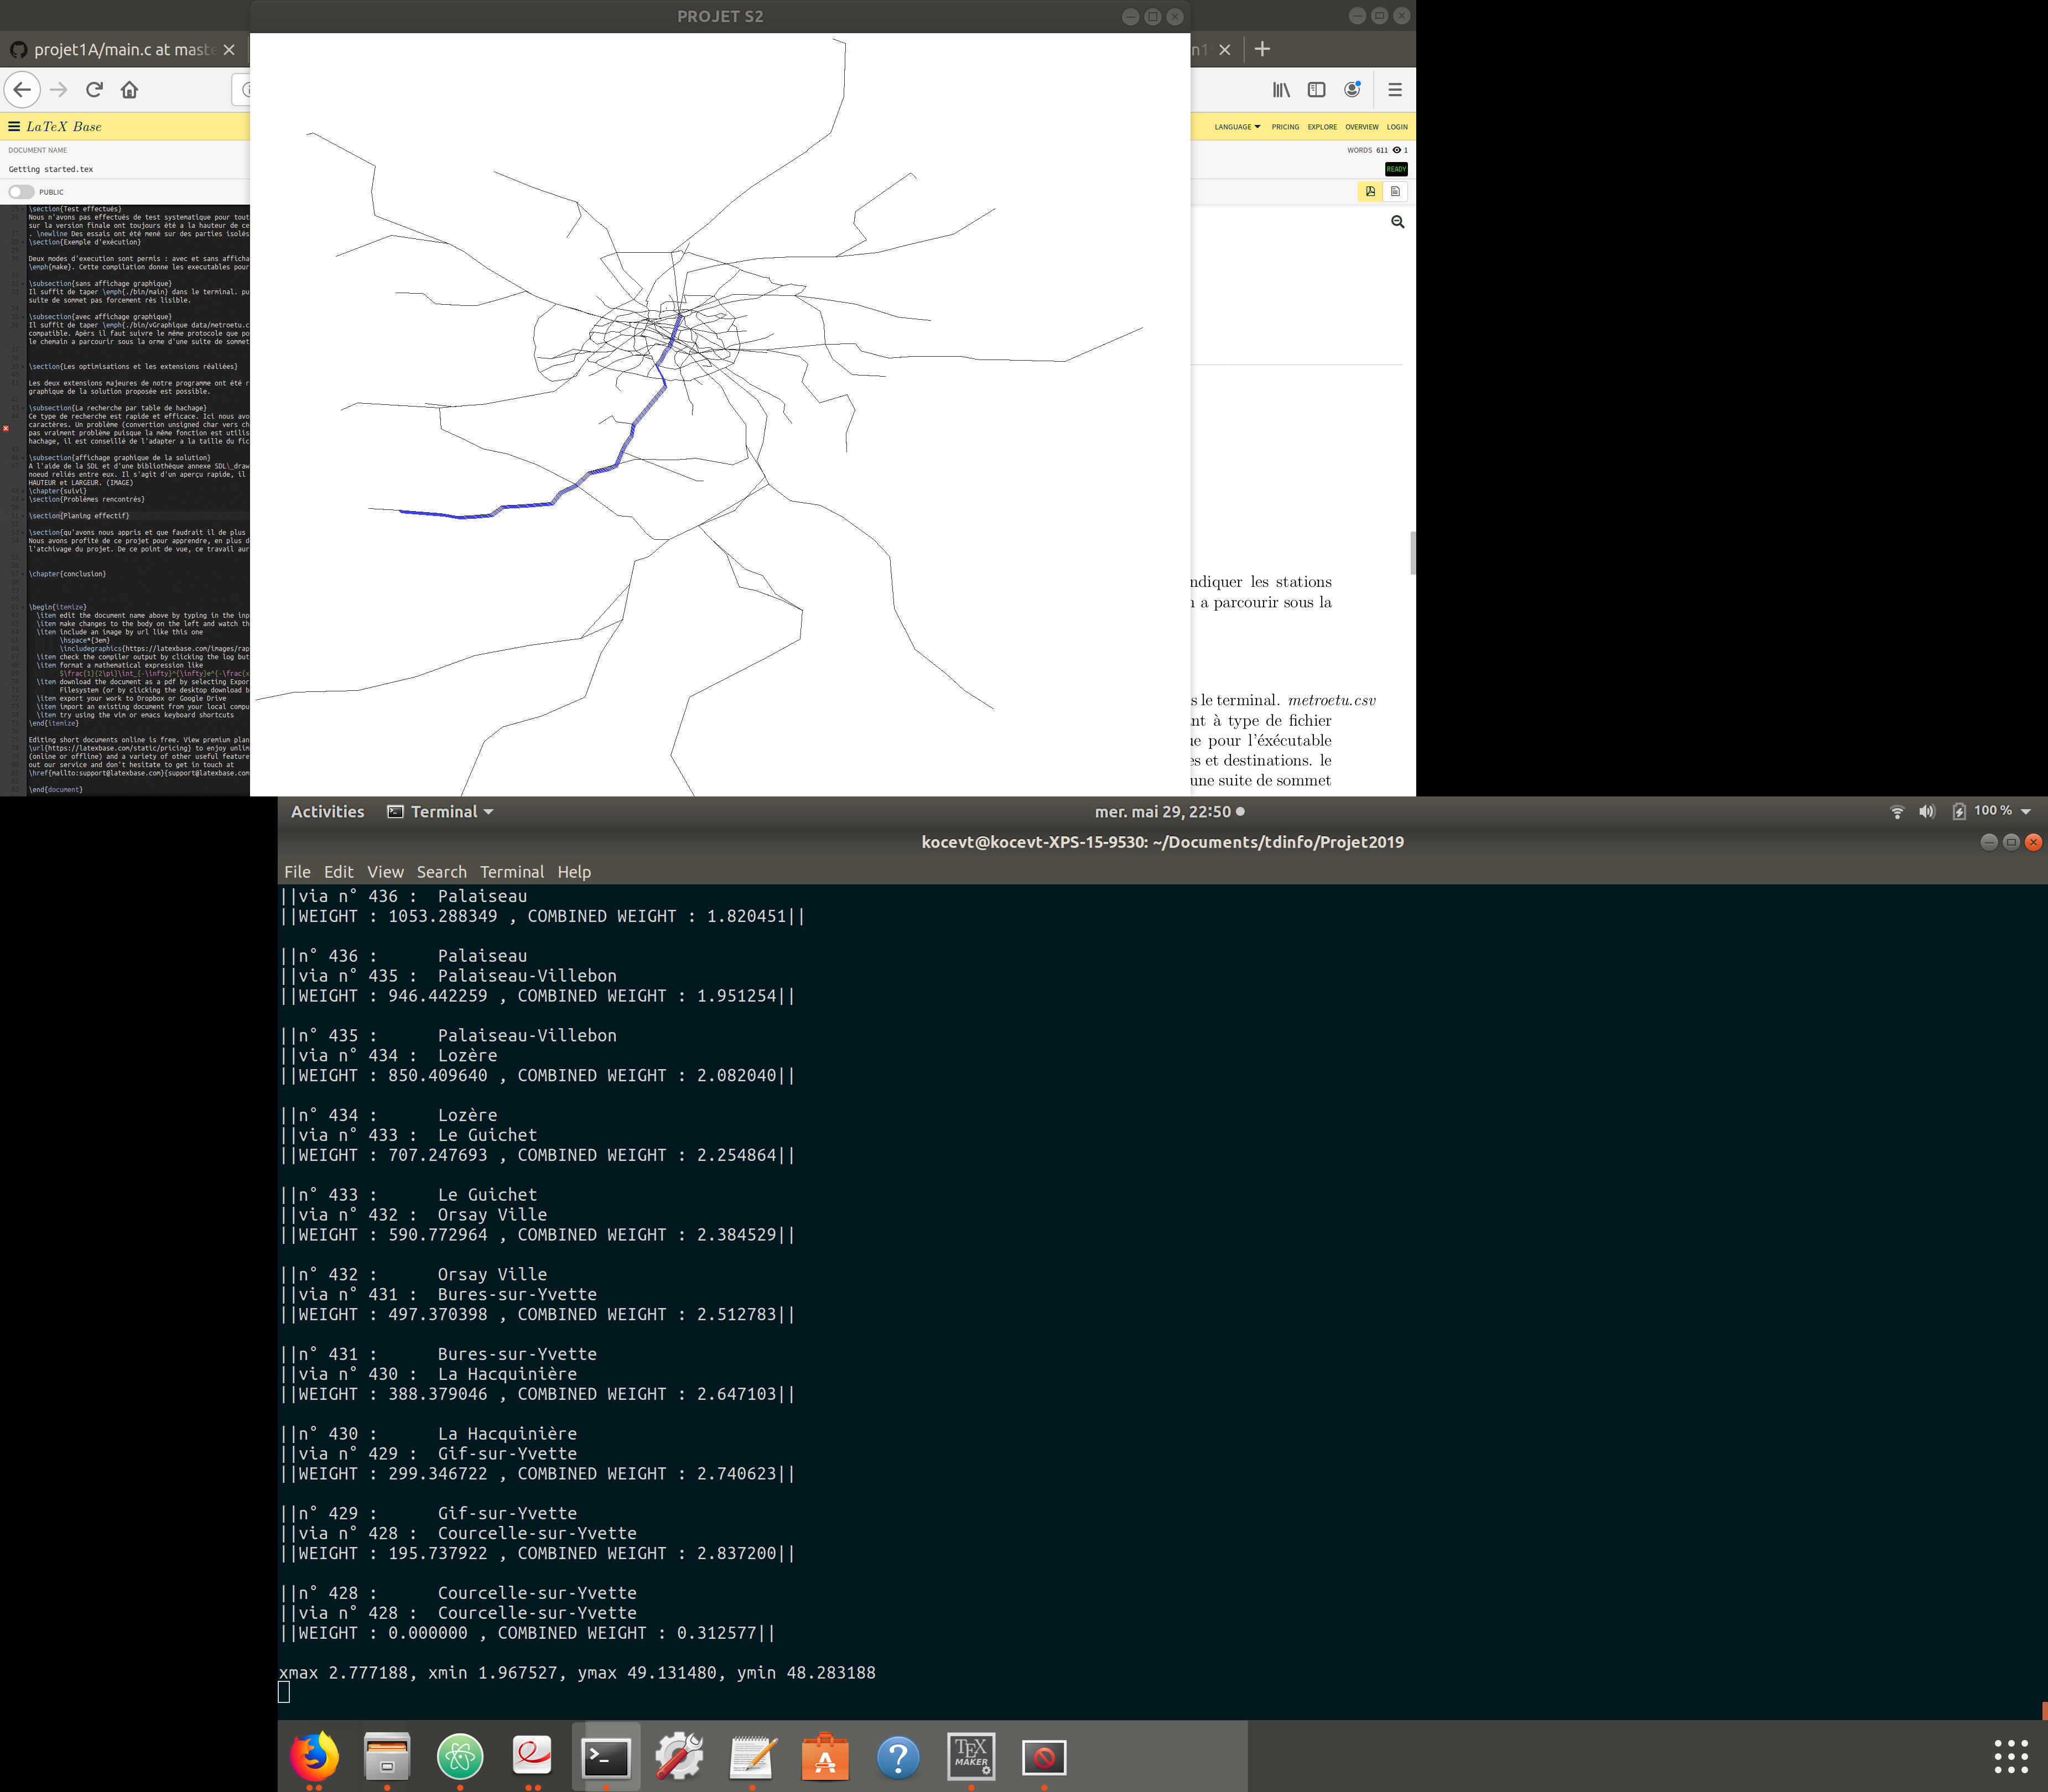
\includegraphics{images/essai.png}

\section{État du logiciel ; ce qui fonctionne, ce qui ne fonctionne pas}
Gobalement nous avons pu avancer jusqu'à la version graphique et la recherche literale par table de hachage est implantée. Il est toujours possible d'obtenir des bugs pour certains sommets qui se trouvent introuvables. \newline Nous avons un problème de libération mémoire. certaines allocations ne sont pas libérées à la fin,et nous n'avons pas eu le temps de regler le problème.
On a aussi un problème pour "doser" les critères de recherche sur le A* car on tend à avoir de meilleurs résultat sur la base de la distance euclidienne plutôt que sur la valeur des arcs.

\section{Tests effectués}
Nous n'avons pas effectués des tests systématiques pour toutes les combinaisons de sommets sur les gros graphes, mais des séries de tests ont été effectuées avec différentes stations. Les résultats sur la version finale ont toujours été a la hauteur de ce que nous espérions à quelques absurditées près, l'itinéraire semble parfois pas tout à fait optimal malgrès des résultats prometteur. Cela semble provenir de l'implantation du A*. 
. \newline Des essais ont été mené sur des parties isolés du programme lors de le conception des différentes parties.
\newline
\newline Un certain nombre de fonctions d'affichage on été implantées et sont d'une aide précieuse
\newline void afficheGraphe(T\_SOMMET*graph, unsigned long len);
\newline void affichetabhach(HACH aff);
\newline void visualiser\_Aliste(ALIST l);
\newline void visualiser\_liste(L\_ARC l);

\section{Exemple d'exécution}

Deux modes d'exécution sont permis : avec et sans affichage graphique. dans les deux cas, il faut se placer dans le répertoire du logiciel et compiler avec la commande \emph{make}. Cette compilation donne les exécutables pour les deux modes.
\newline Il est possible d'avoir des difficultées de compilations pour la version graphique car on a codé avec la SDL sur nos ordinateurs personnels


\subsection{sans affichage graphique}
Il suffit de taper \emph{./bin/main} dans le terminal. puis indiquer les stations origines et destinations. le programme affiche le chemin a parcourir sous la forme d'une suite de sommets dans le terminal. Evidement cette visualisation à ses limites. (figure 1.1)
\newline
\begin{figure}
  \centering
    \includegraphics[width=10cm]{nongraphique.png}
    \caption{Exemple d'itinéraire affiché dans le terminal Depart chatelet, arrivée république}
\end{figure}


\subsection{avec affichage graphique}
Il suffit de taper \emph{./bin/vGraphique data/metroetu.csv} dans le terminal. A noter qu'on peut remplacer \emph{metroetu.csv} par m'importe quel fichier compatible. Après il faut suivre les instructions affichées sur le terminal et entrer en toutes lettres la station d'origines et de destinations. Attention, l'execution est très sensible à la casse et à la ponctuation de part la fonction de hachage. (figure 1.2)\newline
\begin{figure}
  \centering
    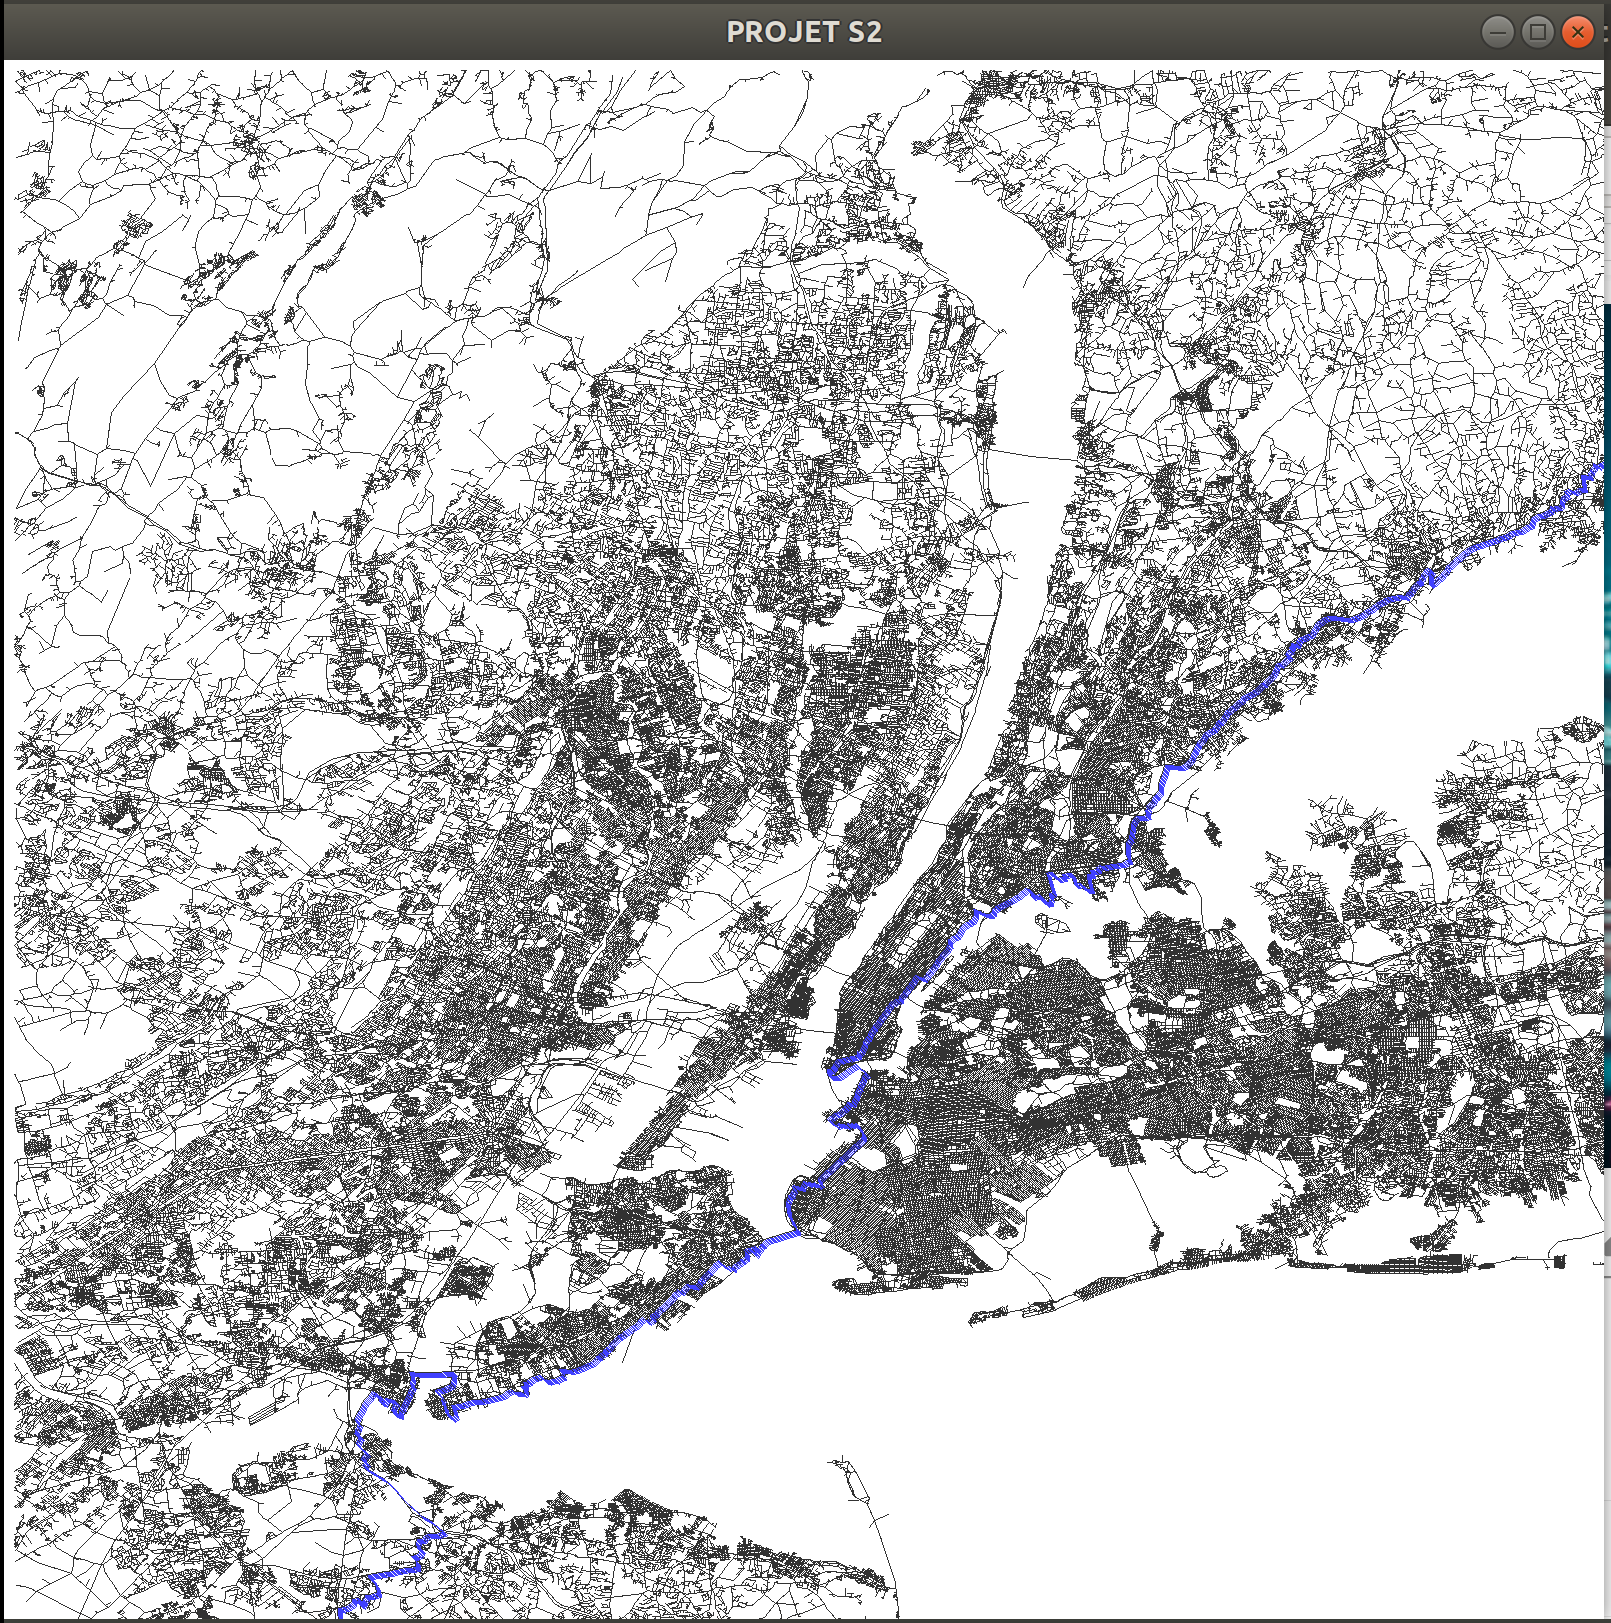
\includegraphics[width=13cm]{Sommets2a80000.png}
    \caption{Intinéraire (en bleu) entre Sommets2 et Sommets80000}
\end{figure}

En bleu on peut voir l'apercu de l'intinéraire entre Sommets2 et Sommets80000

\section{Les optimisations et les extensions réalisées}

Les deux extensions majeures de notre programme ont été réalisées : il est possible de faire la recherche de la station grâce à une table de hachage et un affichage graphique de la solution proposée est possible.

\subsection{La recherche par table de hachage}
Ce type de recherche est rapide et efficace. Ici nous avons fait le choix d'une fonction de hachage particulièrement simple qui ne fait que la somme des valeurs ASCII des caractères. Un problème (conversions unsigned char vers char ?) donnait parfois un hach négatif. Ce problème à été résolu par l'ajout d'une valeur absolue. Chose qui ne pose pas vraiment problème puisque la même fonction est utilisée pour le remplissage et la recherche. Par default la dimension de la table de hachage est le nombre de sommets du graphe. La fonction de hachage utilisée entraine beaucoup de collisions surtout avec le graphe de New York. 

\subsection{affichage graphique de la solution}
A l'aide de la SDL et d'une bibliothèque annexe SDL\_draw on réalise l'affichage des réseaux contenu dans les fichiers. Pour se faire on trace des lignes droite entre chaque noeud reliés entre eux. Il s'agit d'un aperçu rapide, il est possible de modifier l'échelle d'affichage dans graphic.h en modifiant les macros/variables pre-processeur HAUTEUR et LARGEUR. (IMAGE). Une feature intéressante est la mise à l'échelle de la carte quelque soit la résolution choisie à l'aide d'une homotétie. 
\chapter{suivi}
\section{Problèmes rencontrés}

Nous avons rencontrés pas mal de petits problèmes au cours de la réalisation de ce projet, la plus part du temps du a notre faute et au fait que nous avons encore beaucoup à apprendre pour avoir un code efficace. Une difficulté supplémentaire c'est tout de même ajoutée lors de la table de hachage. il y avait pas mal de caractères indésirables sur les lignes des noms des station. Il a aussi fallu trouver une solution pour récupérer une chaîne de caractères avec des espaces. Une première tentative avec \emph{gets} marchait, mais pas sur tous les ordinateurs (fonction dépréciée a partir du C99) on a donc réutiliser \emph{scanf} avec une option pour accepter tous les caractères sauf le retour chariot. Une autre fonction a du être ajouter pour nettoyer un peu le stdin avant la saisie suivante.

\section{Planning effectif}

Nous avons plutôt réussit à bien gérer notre temps, malgré une première séance consacrée à une prise en main un peu longue de GitHub. Une chose très interessante avec GitHub est l'aide à la gestion de projet. Globalement on s'était fixé 4 "Milestones" qu'on a pour la plus-part du temps pas réspectées. Mais ce n'était pas grave car elles étaient ambitieuses et on a toujours pu rattraper sans faire de gros rush\newline
Il n'y a qu'a consulter la rubrique insights du répertoire github https://github.com/BCourteaud76/projet1A pour obtenir un tas d'informations très intéressantes. (notamment sur la distribution de la charge de travail) 
\begin{figure}
  \centering
    \includegraphics[width=13cm]{milestones.png}
    \caption{Milestones sur github}
\end{figure}
\section{qu'avons nous appris et que faudrait-il de plus ?}
Nous avons profité de ce projet pour apprendre, en plus de la gestion des structures de donnée, a utiliser LaTeX pour la rédaction de ce rapport et GitHub pour le partage et l'archivage du projet. De ce point de vue, ce travail aura été d'autant plus instructif et enrichissant.


\chapter{conclusion}

Ce projet nous a pris beaucoup de temps, surtout avec les petites contraintes que nous nous sommes fixées, mais il a été très instructif. De plus ce projet est assez motivant car le logiciel est quand même très proche du quotidien. 

\end{document}
